\documentclass[runningheads]{llncs}
\usepackage{graphicx}
\usepackage{geometry}
\usepackage{lastpage} 
\usepackage{fancyhdr} 
\usepackage{caption}
\usepackage{subfigure}
\geometry{left=2.0cm,right=2.0cm,top=2.0cm,bottom=2.0cm}

\begin{document}
\title{Massive Classification Images Based on Deep Learning Method, Comparing Neural Network, Decision Tree \& Maximum Likelihood}

\author{Hongxiang Zhang\inst{1}}

\authorrunning{Hongxiang Zhang}

\institute{
	Research School of Computer Science	Australian National University\\
	\email{u7101924@anu.edu.au}
}
%
\maketitle
%
\begin{abstract}
Deep learning method has become a hotspot topic in recent years, which achieves remarkable performance in many machine learning fields. In the real world, massive classification has a wide application. In this paper, we focus on using the deep learning method to abstract features from images and then compare neural networks, decision tree, and maximum likelihood in classification[1].

In this paper, we choose VehicleX-v2[2] as the dataset, which contains various vehicle images. The dataset was separated into train, validation, and test sets, which have 45438, 14936, and 15142 images respectively. Each image is 256*256 with RGB channels. And, to solve the massive classification, we propose different data augmentation functions to avoid overfitting, and various methods to improve the performance.

After comparing different network structure and hyper-parameters combination, we propose a brand new network based on VGG network[3] followed by neural network classifier, which achieves 75.09\% accuracy on test set and 96.50\% on train set.

\keywords{Massive Classification  \and Deep learning \and Convolutional Neural network \and decision tree \and maximum likelihood.}

\end{abstract}

\section{Introduction}

Massive classification has become an essential part in many real-world systems, for example medical, Big data technology, including artificial intelligence. The performance of massive classification plays an important role on these tasks. In this paper, we aim to find the best solution for massive classification on image dataset.

VehicleX-v2 was chosen as our dataset which has a large-scale synthetic vehicle images containing 1362 vehicles. Created in Unity, VehicleX-v2 combine the synthetic vehicle model and real-world vehicle re-ID datasets, it not only has a high degree of reality but also editable on a specific attribute. Each image in the dataset is one vehicle at an angle and shaped with 256*256 in RGB channels. The dataset was divided into train set, validation set, and test set with 45438, 14936, and 15142 images respectively. Facing this large-scale dataset, various data augmentation and data preprocessing methods were applied to improve the performance.

In this paper, we aim to use the deep learning method to extract features from the dataset and compare different methodology to classify the vehicle-ID which is 1,362 classes. Our experimental strategy is to implement a deep convolutional network as feature extractor to get features, then compare different classifiers, which implement by neural network, decision tree, and maximum likelihood. The model was trained with train-set showing the accuracy and loss, also adjust hyper-parameters with validation set. Finally, Using test set to show the accuracy and loss to evaluate the model. The result suggests that deep learning method and neural network classifier achieve a remarkable performance on massive classification, and multiple convolutional layer network performs well on extract features from images. However, overfitting still exists in this network. Based on those findings, we conclude and apply serious techniques to avoid overfitting and improve performance.

\section{Method}
We introduce a new convolutional neural network to extract features and classify the images. A large-scale synthetic dataset named VehicleX-v2 was chosen as the dataset, which has a diverse range of realistic backbone models and textures. Also, we present various data augmentation methods and data preprocessing methods to improve the performance. At the same time, we have applied and concluded techniques to avoid overfitting in deep learning network. Taken together, our experiments show a result that the best way to solve massive Classify Images.

\subsection{Data Augmentation \& Data Processing}

VehicleX-v2 has a diverse range of realistic backbone models and textures, allowing it to be able to adapt to the variance of real-world datasets[2]. In this paper, we aim to find the best network structure to solve massive classification in images, before this data augmentation and data preprocessing is an essential task to do. In VehicleX-v2 dataset, all images were separated into train-set, test-set, and validation set with 45,438, 15,142, and 14,936 files respectively. To speed up file loading time, all labels were stored in "npy" files. For label files, each line represents one image in the dataset, the first column represents the file path, and the second column is the label that the image belongs to. And there are 1326 classes in total.

Each image in dataset can represent by [256*256*3] matrix, which indicates R, G, B channels in 256 height and 256 widths. As shown in Figure~\ref{fig1}, randomly flip the image, and transfer the image to tensor. Different augmentation methods are applied to augment the data. And from our experiment, it can reduce the overfitting in an efficient way.
\begin{figure}
	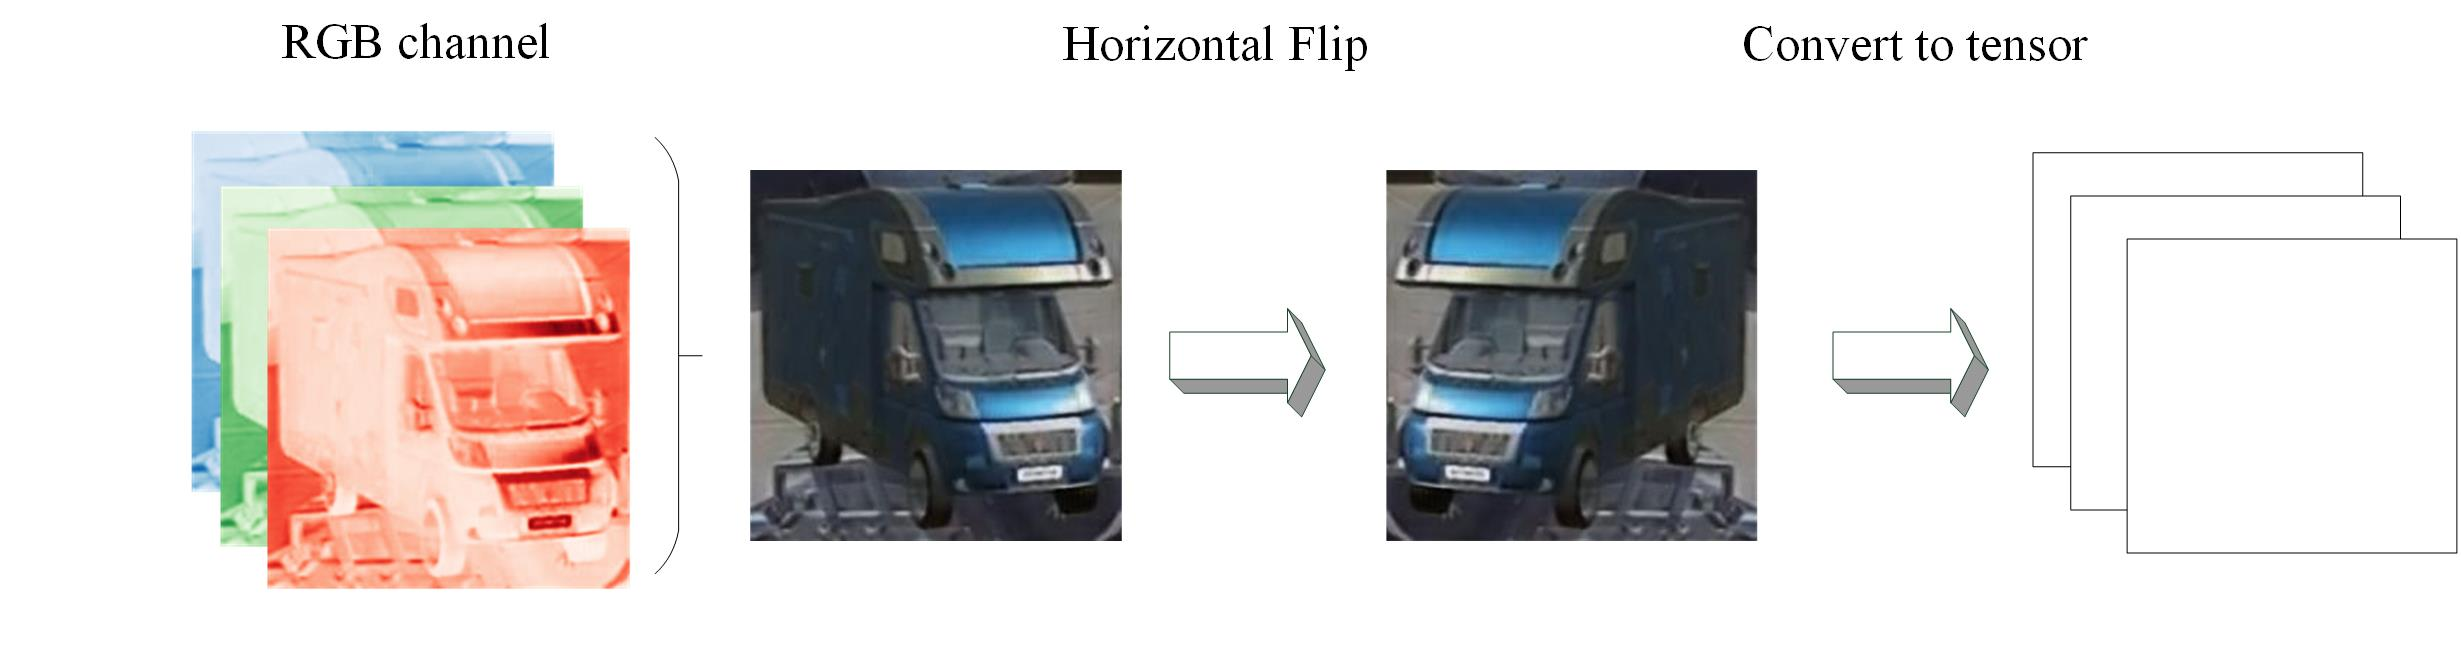
\includegraphics[width=\linewidth]{augmation.jpg}
	\caption{Data augmentation and data preprocessing. Each image has R,G,B channel, and randomly horizontal flipped, then transferred to tensor to boost computation}
	\label{fig1}
\end{figure}

In the dataset, different images have diverse value ranges which may affect the performance of classification. In this case, we applied normalization[4] to reduce this effect.

Normalization: For each image $i$, subtract the mean image of the whole dataset, then divide by the standard difference of the whole dataset. $mean$ represent the mean image of the whole dataset, $std$ indicate the standard difference of the whole dataset.
\begin{equation}
	Normalized_i=\frac{image_i-mean}{std}
\end{equation}

Normalization is an efficient way to reduce the bad effect of different value ranges. At the same time, normalization makes different dimension feature comparable. From our experiment, it can improve the accuracy of the model.

\subsection{Deep Learning}
In this paper, We propose a new deep learning neural network based on VGG net[3] to extract features and classify the images. The architecture of the model consists of two parts - a convolutional neural network for extract features and a fully connected neural network to learn the features followed by a softmax layer for classification.

As illustrated in Figure~\ref{fig2}, convolutional neural network takes in all input images. Convolutional kernel is able to extract features from images then output the feature map. Followed by max-pooling layer, which able to retain the main feature like edges, scale in the image, and reduce parameters and calculation in the next layer. Also, pooling can avoid overfitting in some degree. As shown on the above graph, conv3 and conv4 are followed by an activation function. After convolutional neural network extract features, the feature was reshaped to one dimension, then passed to the fully connected neural network. Fully connected layer connect every neural to every activation unit in the next layer, which is able to synthesize the features extracted from the upper layers. The output of the fully connected layer pass to the softmax layer for classification. Softmax layer generally used for classification, which mapping the features into range$[0,1]$ of each category. The output represents the probability of each class.
\begin{figure}
	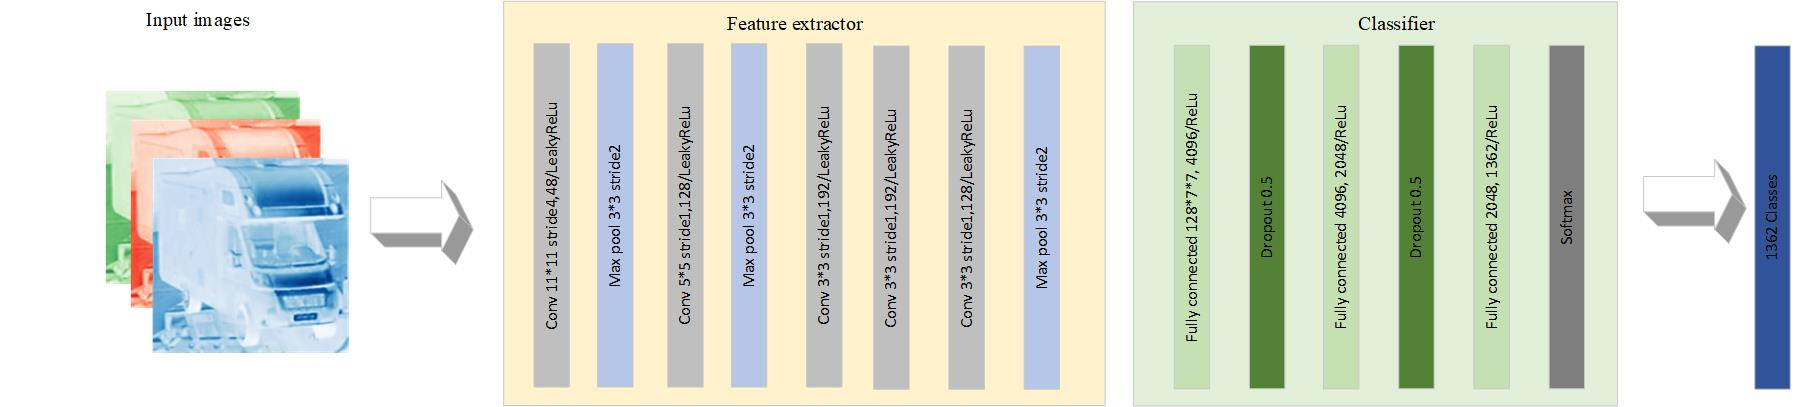
\includegraphics[width=\linewidth]{network.jpg}
	\caption{Illustrate the network structure. There are 5 convolutional layer with 3 max pooling layer in feature extractor, 3 fully connected layer in classifier.} \label{fig2}
\end{figure}

\subsubsection{Convolutional layer}
Convolutional layers[5] convolve the input to a feature map. Each convolutional layer was defined by convolutional kernel, padding, and stride. After convolution operation, input will be abstract to a feature map. Equation 2 represents the operation of convolution.
\begin{equation}
	f(x_i)=\frac{\sum_{j=0}x_j*kernel_j}{kernel.size}
\end{equation}

\subsubsection{Max pooling layer}
Max pooling layer replaces the value with the max value in a kernel, which provides an abstract form of representation to reduce the parameters and computational cost. Equation 3 represents the operation of max pooling.
\begin{equation}
	f(x_i)=max(X) X\in kernel
\end{equation}

\subsubsection{Fully connected layer}
Each fully connected layer consists multiple neural. As illustrated in Figure~\ref{fig3}, fully connected layer takes features as input, each dimension in features corresponding to one neural[5]. These two Fully connected layer are denoted as $FC_1$ and $FC_2$ with $n_1$ and $n_2$ neural respectively. Assume x be one output of layer$FC_1$, where $x$ belongs to $R^{{n_1}*1}$. And $W$ be the weight matrix of $FC_2$, where $W$ belongs to $R^{{n_1}*{n_2}}$. Each column $w_i$ in $W$ is the weight vector corresponding to $i$th neuron in $FC_2$. In this case, $W^T*x$ is the output of $FC_2$. This operation compiles the data extracted by convolutional layer to generate the final output.

\begin{figure}
	\centering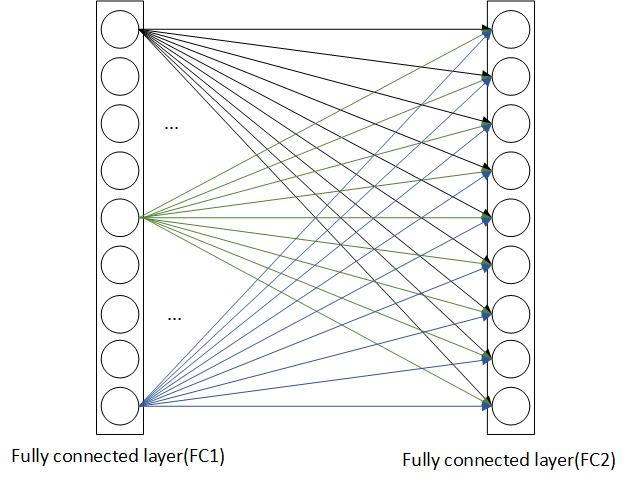
\includegraphics[width=8cm]{fc.jpg}
	\caption{Illustrate of FC, n1, n2 stands for the number of neurons in FC1, FC2 respectively} \label{fig3}
\end{figure}


\subsubsection{Activation Function}
The activation function is a non-linear function that can enhance the neural network and map the input to region $[0,1]$. In our model, we choose LeakyReLu as activation functions[6]. As shown in Figure~\ref{fig4}. LeakyReLu has a good performance on computation, when the input is positive LeakyRelu will not have trouble with gradient explosion. Also, when input is negative Leaky Relu still responds to the input.
\begin{equation}
	LeakyReLu(z)=max(\alpha x,x)
\end{equation}

\begin{figure}
	\centering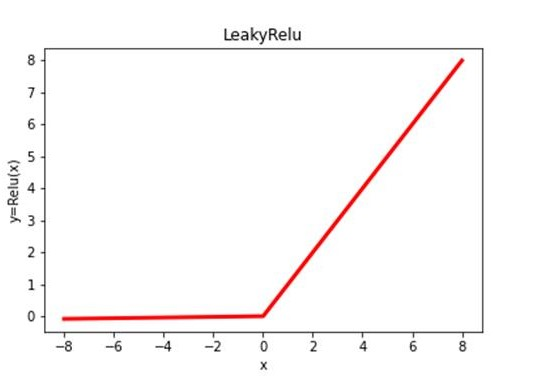
\includegraphics[width=7cm]{leakyrelu.jpg}
	\caption{graph represent the activation function graph LeakyRelu} \label{fig4}
\end{figure}

\subsubsection{Softmax layer}
Softmax layer widely applied to classification, which mapping the input to range $[0,1]$ of each category. Each dimension is the probability of each class. As illustrated in Figure~\ref{fig5}. Assume $V$ is the input vector of softmax layer, $z_i$ represent the $i$th category value in $V$, the output of the $i$th category is $y_i$.
\begin{equation}
	y_i=\frac{e^{z_i}}{\sum_j e^{z_j}}
\end{equation}

\begin{figure}
	\centering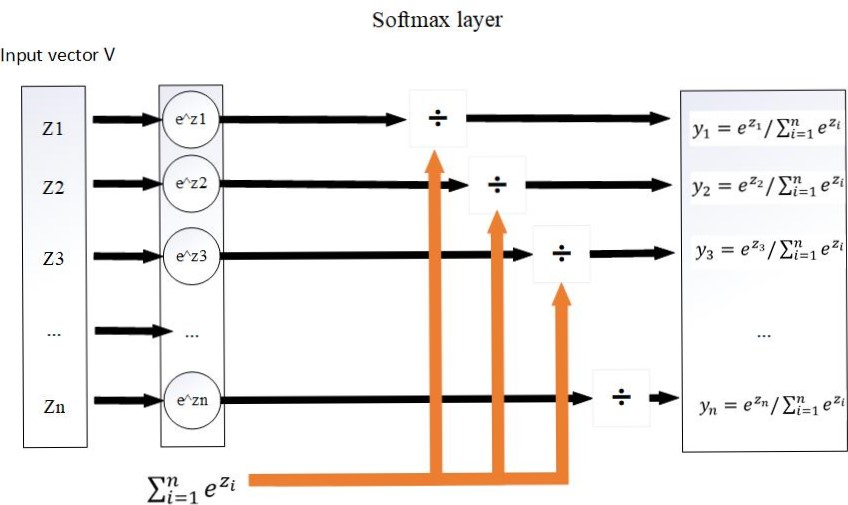
\includegraphics[width=10cm]{softmax.jpg}
	\caption{Illustration of the softmax calculation process. After calculation, each input is map to range$[0,1]$.}
	\label{fig5}
\end{figure}

\subsection{Decision Tree}
A Decision Tree is a divide and conquers method to classification, which widely used in discover features in a large dataset. Decision Tree uses the branch structure to classify each feature vector into categories[7]. Shannon[8] introduces Entropy which represents the amount of eliminating the uncertainty. It was written as
\begin{equation}
	Entropy(t)=-\sum_{i=0}^{c-1}p(i|t)\log_2p(i|t)
\end{equation}
Which $p(i|t)$ represents the probability that node t belongs to class i. When the uncertainty is greater, It needs a larger amount of information and greater entropy. Also, Higher entropy represents lower purity which means when the dataset is evenly mixed, the entropy is the greatest with the lowest purity. In this paper, we build a decision tree based on purity. ID3 algorithm is an effective way to improve purity, which calculates entropy in each node. Written as
\begin{equation}
	Gain(D,a)=Entropy(D)-\sum_{i=1}^{k}\frac{|D|}{|D_i|}Entropy(D_i)
\end{equation}



\subsection{Maximum Likelihood}
Maximum Likelihood classification is a statistically based method derived from Bayes theorem, which is commonly used in traditional classification. It mainly uses a discriminant function to classify each pixel to the class with the highest likelihood [9]. This paper uses each feature value in an feature vector to identity the feature vector to the corresponding class. Let $P(i|\omega)$ as the posterior distribution, $i$ is the $i$th class, $\omega$ is the feature vector.
\begin{equation}
	P(i|\omega)=\frac{P(\omega|i)P(i)}{P(\omega)}
\end{equation}
$P(\omega|i)$represent the likelihood function, and $P(i)$ is a priori information. In this case, The probability of $\omega$ is

\begin{equation}
	P(\omega)=\sum_{i=1}^{M}P(\omega|i)P(i)
\end{equation}


\section{Results and Discussion}

In this paper, dataset was separated into train set, test set, and validation set with 45438, 15142, 14936 images respectively. 60\% of identities are used for training, 20\% for testing, the other 20\% are used for adjusting parameters. The challenge in this data set is that the massive amount of data. To apply our model, all data are being normalized, randomly flipped, rearrange the order, and convert to the tensor which boosts computing[10]. During the experiment, we also use CUDA to accelerated computation. We applied and concluded a series of network architecture and hyper-parameters to improve performance and compare three classification methods. For all experiments, the model was trained with the same train set and evaluate with the same test set.

\subsection{Feature extractor}
\subsubsection{Network Architectural}
In this task, we compare two network architectural both based on VGG network[3]. Both of them are train and test in the same dataset, also we use the same three-layer neural network as classifier to compare the performance. As illustrated in Figure~\ref{fig6}. The first network contains three convolutional layers followed by LeakyReLu activation functions, compared with the second network which has five convolutional layers. These two networks are trained and evaluated in the same dataset and using the same classifier.

\begin{figure}[htbp]
	\centering
	\subfigure[Network a]
	{
			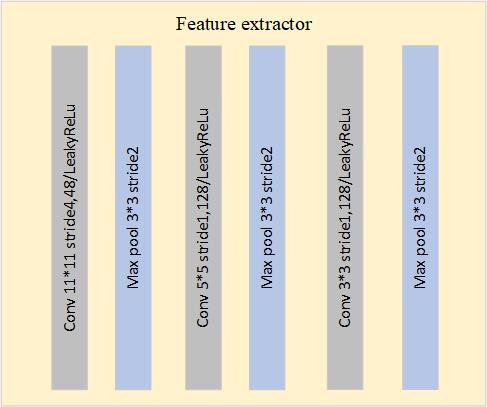
\includegraphics[width=6.4cm]{stru1.jpg}
	}
	\subfigure[Network b] %第二张子图
	{
			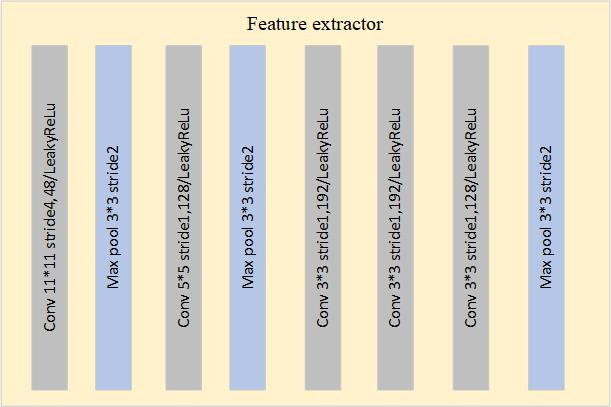
\includegraphics[width=8cm]{stru2.jpg}
	}
	
	\caption{Illustration of the two different feature extractor. Network a consists 3 convolution layer compare with 5 convolution layer in Network b. They both train and test in the same dataset. And followed by a neural network classifier.}
	\label{fig6}
\end{figure}


As illustrate in Figure~\ref{fig7}, network b performs better, which achieves over 75\% accuracy on test set and over 95\% accuracy on train set. network a achieve over 65\% accuracy on test set and over 95\% accuracy on train set. It is clear to see that network a is more overfitting than network b, at the same time, when trained in the same epochs it performs not as good as network b. what else, from subfigure c d show, the loss in network b descend faster. It is easy to understand why, for network a, which has a shallow network may not able to extract sufficient features from images. In this case, it will get overfitting. Compared with the deep one, the loss descent faster and perform better. But it still has a problem with overfitting, which is widely appeared in deep learning networks. In future studies, we will try different network structures to reduce overfitting, for example, shortcut connection in ResNet[11].


\begin{figure}[htbp]
	\centering
	\subfigure[Accuracy of network a]{
		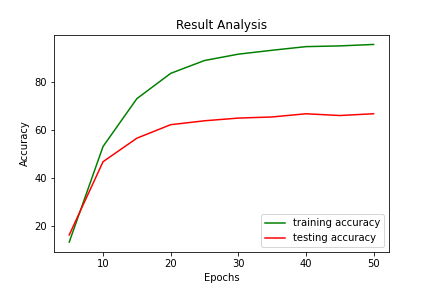
\includegraphics[width=7cm]{result1.png}
		%\caption{fig1}
	}
	\quad
	\subfigure[Accuracy of network b]{
		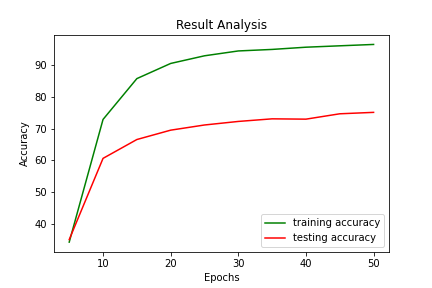
\includegraphics[width=7cm]{result2.png}
	}
	\quad
	\subfigure[Loss of network a]{
		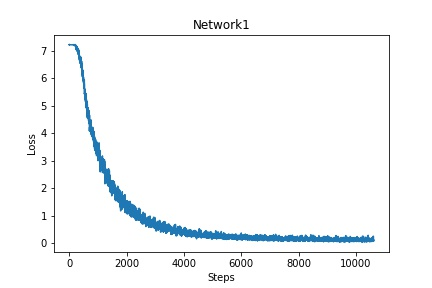
\includegraphics[width=7cm]{loss1.jpg}
	}
	\quad
	\subfigure[Loss of network b]{
		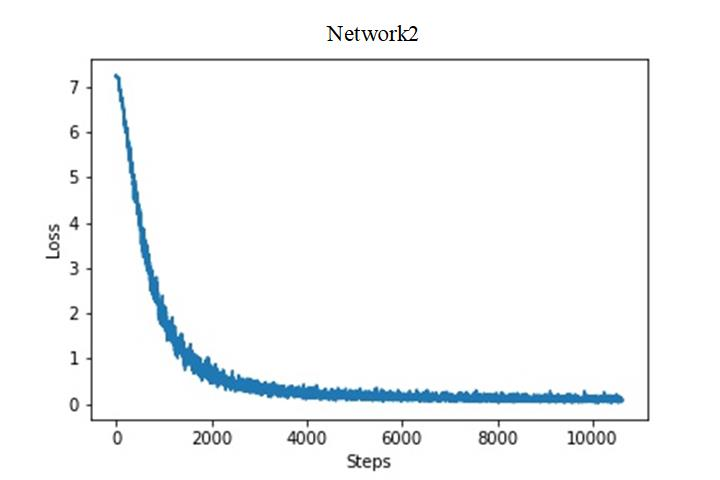
\includegraphics[width=7cm]{loss2.jpg}
	}
	\caption{Illustration of the accuracy and loss on network a and b.}
	\label{fig7}
\end{figure}

\subsubsection{Hyper parameters}
Hyper parameters play an important role in a neural network, especially in deep learning. Different combinations of hyper parameters leads a diverse result in a model. In this task, we aim to compare different combinations of learning rates and epochs to find the best hyper parameters. Compare Adam[12] and SGD[13], SGD with stochastic character may converge slower than other gradients descends method, and it may oscillate at the saddle point, also SGD is not able to dynamically adjust learning rate, which may not able to reach the minimum point at the end of training. In contrast, Adam combines RMSprop and Momentum, which auto-adjust learning rate and add momentum to the direction of gradient descend to speed up gradient descent. Also, batch size is another factor that affects the convergence speed. Generally, models with larger batch size need less computation cost and converge faster. Considering the size of dataset, and after several times of training, we choose batch size at 256, network b as our model, and Adam as our optimizer. Table~\ref{tab2} gives a summary of choosing Hyper parameters.

\begin{table}
	\caption{Comparesion between Learning rate, epoches and optimiser}\label{tab2}
	\begin{center}
		\begin{tabular}{|l|l|l|l|l|}
			\hline
			Learning rate & Epochs & Final Loss & Train set Accurcy & Test set Accurcy\\
			\hline
			0.005 & 20 & 7.2361 & 0.06\%  & 0.06\%\\
			0.005 & 30 & 7.2680 & 0.10\%  & 0.09\%\\
			0.005 & 50 & 7.1987 & 0.08\%  & 0.04\%\\
			\hline
			0.0005 & 20 & 0.2507  & 89.73\%  & 68.70\%\\
			0.0005 & 30 & 0.2922  & 93.11\%  & 71.73\%\\
			0.0005 & 50 & 0.1595  & 94.67\%  & 73.83\%\\
			\hline
			0.0003 & 20 & 5.2364  & 90.51\%  & 69.48\%\\
			0.0003 & 30 & 3.3942  & 94.45\%  & 72.25\%\\
			0.0003 & 50 & 0.1281  & 96.50\%  & 75.09\%\\
			\hline
		\end{tabular}
	\end{center}
\end{table}

From the table above, hyper parameters with 0.0003 learning rate, 50 epoch, and 256 batch size perform best in the model. Learning rate is an essential factor that affects the performance of the model. As Figure~\ref{fig8} illustrates, when learning rate is 0.01, loss keeps at a high level around 7, which show that learning rate is too high that gradient always descent overhead and it can not reach the minimum point. Compare 0.0005 and 0.0003, 0.0003 perform better at the beginning of the training and have a better performance in the end. For epochs, loss descent under 1 when epochs are 50, and the accuracy achieves the highest mark in both train and test set.
\begin{figure}[htbp]
	\centering
	\subfigure[learning rate 0.005]
	{
		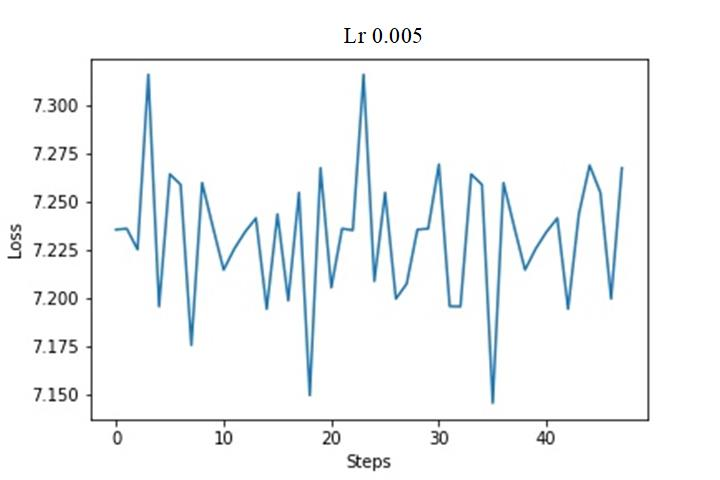
\includegraphics[width=5cm]{Loss3.jpg}
	}
	\subfigure[learning rate 0.0005] %第二张子图
	{
		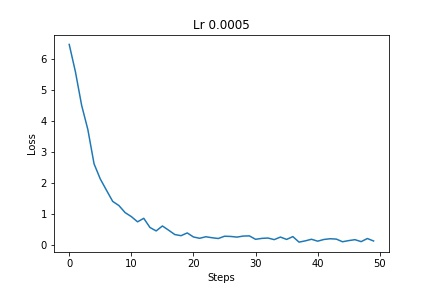
\includegraphics[width=5cm]{Loss4.jpg}
	}
	\subfigure[learning rate 0.0003] %第二张子图
	{
		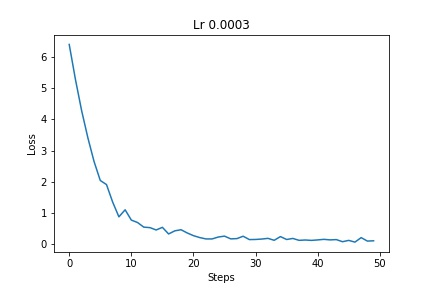
\includegraphics[width=5cm]{Loss5.jpg}
	}
	\caption{Illustration of loss in learning rate at 0.005, 0.0005, and 0.0003 respectively}
	\label{fig8}
\end{figure}

\subsection{Classifier}
\subsubsection{Neural Network}
In this task, we choose three-layer neural network as our classifier. The input is the feature map extracted by last convolutional layer. Each fully connected layer was followed by a dropout layer. Finally softmax layer map the feature to each classes. As shown in table~\ref{tab3}. Neural Network achieves a remarkable performance on both train set and test set. We can conclude that the Neural network is an appropriate classifier for the massive classification.
\begin{table}
	\caption{Neural Network Performance }\label{tab3}
	\begin{center}
		\begin{tabular}{|l|l|l|l|}
			\hline
			& Correct & False & Accuracy\\
			\hline
			Train set &  43847  &  1591   & 96.50\% \\
			Test set  & 11370   &  3772   & 75.09\%\\
			\hline
		\end{tabular}
	\end{center}
\end{table}


\subsubsection{Decision Tree}
In this session, we use the ID3 algorithm to implement Decision Tree for classification. Due to the massive class in this paper, the Decision tree in this task has a huge amount of branches for decisions. As shown in the table~\ref{tab4}, It is unusual to achieve better performance on this dataset. Due to the Massive amount of classes, this decision tree is much complex and redundant, which means there is a small difference between each class, which leads to a bad performance on the Decision tree. In this case, our conclusion is that the Decision Tree is not a proper method for massive classification.

\begin{table}
	\caption{Decision Tree Performance }\label{tab4}
	\begin{center}
		\begin{tabular}{|l|l|l|l|}
			\hline
			          & Correct & False & Accuracy\\
			\hline
			Train set &  5707  &   39731   & 12.56\% \\
			Test set  &  67    &   15075   & 0.44\%\\
			\hline
		\end{tabular}
	\end{center}
\end{table}

\subsubsection{Maximum Likelihood}
For Maximum Likelihood, we choose Multinomial Naive Bayes for classification, which assumes probability distribution obeys a multinomial. For this massive classification task, we need to calculate the prior probability and conditional probability of each data to each class, then using these probabilities to estimate the class. As the table~\ref{tab5} shown, Multinomial Naive Bayes did not perform well on both the training set and test set. We can infer that simple Multinomial Naive Bayes can not fully learn the features for classification.

\begin{table}
	\caption{Maximum Likelihood Performance }\label{tab5}
	\begin{center}
		\begin{tabular}{|l|l|l|l|}
			\hline
			& Correct & False & Accuracy\\
			\hline
			Train set &  5707  &   39731   & 29.00\% \\
			Test set  &  67    &   15075   & 6.00\%\\
			\hline
		\end{tabular}
	\end{center}
\end{table}

\subsection{Summary and Discussion}
Due to the limitation of computations and after comparing different network architecture for feature extractor and three methods for classifier: Neural Network, Decision tree, and Maximum likelihood. We got conclude that 5-layer convolutional network based on VGG and Neural network for classification is the best combination for massive classification. In the previous experiments, we have discussed different architectural and hyper parameters for feature extractors. However, accuracy on train set is still much higher than the accuracy on the test set. We have tried serious of methodology to avoid overfitting, for example, dropout, rearrange the order. Also, there are multiple methods to improve the performance on test set. Shortcut connection in ResNet is an interesting structure that may able to avoid overfitting efficiently. Also, comparing with the state-of-art performance[2], which achieve 85.72\%mAP, there is still a place for improvement. From the experiment data we collected, we guess a deeper and more complex neural network might able to improve the performance to a higher level.

The traditional methods like Decision trees and maximum likelihood did not achieve ideal performance. The Decision tree produces the worse results on both train-set and test-set. Facing massive classification, the Decision tree needs huge number of branches to classify each data which is low efficiency and bad performance. And if the algorithm make the wrong decision at the beginning, the result would deviate the ground truth label. The maximum likelihood which based on statistical theory can have a good performance on normal classification, but faced with massive feature map in each classes, maximum likelihood performed not well. We got to conclude that decision tree and maximum likelihood are not the appropriate methods for massive classification.

\section{Conclusion and Future Work}
In this paper, we propose a deep neural network based on VGG to extract features and evaluate three methods for classification. First, we developed different architecture in the Neural network. These models are trained and evaluated with the same dataset. After the experiment, we found 5-layer convolutional neural network performs best, which achieves 75.09\% accuracy on test set. Then, we compare three methods for classification, results show that the Neural Network model outperforms compared to the traditional methods. While in this paper, we also discuss different ways to optimize the model, and the model achieves ideal performance finally. But there still amount of ways to improve the performance, extended dataset, deeper network, more advanced structure.

Due to the limitation of computer performance and research time, there are also other models and techniques for classification, for example, speed up SVM algorithm[14], shortcut connection structure in ResNet[11], and deeper feature extractor, for example, ResNet[11], Google Net[15]. According to the paper, Speed up SVM achieves great performance on massive classification. And shortcut connection is an interesting and efficient method to avoid overfitting and improve performance. We will explore those techniques in the future.

\section{Reference}

\quad 
[1]Milne, L. K., Gedeon, T. D., \& Skidmore, A. K. (1995). Classifying Dry Sclerophyll Forest from Augmented Satellite Data: Comparing Neural Network, Decision Tree \& Maximum Likelihood. training, 109(81), 0.\\

[2]Yao, Y., Zheng, L., Yang, X., Naphade, M., \& Gedeon, T. (2019). Simulating content consistent vehicle datasets with attribute descent. arXiv preprint arXiv:1912.08855.\\

[3]Simonyan, K., \& Zisserman, A. (2014). Very deep convolutional networks for large-scale image recognition. arXiv preprint arXiv:1409.1556.\\

[4]Jayalakshmi, T., \& Santhakumaran, A. (2011). Statistical normalization and back propagation for classification. International Journal of Computer Theory and Engineering, 3(1), 1793-8201.\\

[5]Ma, W., \& Lu, J. (2017). An equivalence of fully connected layer and convolutional layer. arXiv preprint arXiv:1712.01252.\\

[6]Ramachandran, P., Zoph, B., \& Le, Q. V. (2017). Searching for activation functions. arXiv preprint arXiv:1710.05941.\\

[7] Myles, A. J., Feudale, R. N., Liu, Y., Woody, N. A., \& Brown, S. D. (2004). An introduction to decision tree modeling. Journal of Chemometrics: A Journal of the Chemometrics Society, 18(6), 275-285.\\

[8] Bromiley, P. A., Thacker, N. A., \& Bouhova-Thacker, E. (2004). Shannon entropy, Renyi entropy, and information. Statistics and Inf. Series (2004-004).\\

[9] Strahler, A. H. (1980). The use of prior probabilities in maximum likelihood classification of remotely sensed data. Remote sensing of Environment, 10(2), 135-163.\\

[10]Shorten, C., \& Khoshgoftaar, T. M. (2019). A survey on image data augmentation for deep learning. Journal of Big Data, 6(1), 1-48.\\

[11]He, K., Zhang, X., Ren, S., \& Sun, J. (2016). Deep residual learning for image recognition. In Proceedings of the IEEE conference on computer vision and pattern recognition (pp. 770-778).\\

[12] Kingma, D. P., \& Ba, J. (2014). Adam: A method for stochastic optimization. arXiv preprint arXiv:1412.6980.\\

[13] Bottou, L. (2010). Large-scale machine learning with stochastic gradient descent. In Proceedings of COMPSTAT'2010 (pp. 177-186). Physica-Verlag HD.\\

[14] Do, T. N., Nguyen, V. H., \& Poulet, F. (2008, October). Speed up the SVM algorithm for massive classification tasks. In International conference on advanced data mining and applications (pp. 147-157). Springer, Berlin, Heidelberg.\\

[15]Szegedy, C., Liu, W., Jia, Y., Sermanet, P., Reed, S., Anguelov, D., ... \& Rabinovich, A. (2015). Going deeper with convolutions. In Proceedings of the IEEE conference on computer vision and pattern recognition (pp. 1-9).\\

\end{document}
